
\title{Recap Information Systems (01PDWOV)}
\author{Jacopo Nasi\\
        Computer Engineer\\
        Politecnico di Torino}
\date{I Period - 2018/2019\\\bigskip\bigskip\today}

\documentclass[12pt]{article}
\usepackage[utf8]{inputenc}
\usepackage[english]{babel}
\usepackage{geometry}
\usepackage{indentfirst} % First line indent
\usepackage{mathtools}
\usepackage{wrapfig}
\usepackage[usenames, dvipsnames]{color}
\usepackage{float}
\usepackage{amssymb}
\usepackage{ifsym}
\usepackage{listings}
\usepackage{multicol}

% Misure Documento
\geometry{ a4paper, total={170mm,257mm},left=35mm, right=35mm, top=35mm, bottom=35mm }

\begin{document}

\begin{figure}
  \centering
  
\includegraphics[width=10cm]{images/polito.pdf}
\end{figure}

\maketitle


\newpage
\tableofcontents

\newpage
{\noindent \Large \textbf{License}\bigskip}

This work is licensed under a Creative Commons Attribution-NonCommercial-ShareAlike 3.0 Unported License.\\
You are free:
\begin{itemize}
  \item \textbf{to Share}: to copy, distribute and transmit the work
  \item \textbf{to Remix}: to adapt the work
\end{itemize}
Under the following conditions:
\begin{itemize}
  \item \textbf{Attribution}: you must attribute the work in the manner specified by the author or licensor (but not in any way that suggests that they endorse you or your use of the work)
  \item \textbf{Noncommercial}: you may not use this work for commercial purposes.
  \item \textbf{Share Alike}: if you alter, transform, or build upon this work, you may distribute the resulting work only under the same or similar license to this one.
\end{itemize}

\noindent More information on the Creative Commons website (http://creativecommons.org).

\begin{figure}[h!]
  \centering
  
\includegraphics[width=3cm]{images/license.png}
\end{figure}

{\noindent \Large \textbf{Acknowledgments}\bigskip}

Questo breve riepilogo non ha alcuno scopo se non quello di agevolare lo studio di me stesso, se vi fosse di aiuto siete liberi di usarlo.\\
Le fonti su cui mi sono basato sono quelle relative al corso offerto (\textbf{Information Systems (01PDWOV)}) dal Politecnico di Torino durante l'anno accademico 2018/2019.\\
Non mi assumo nessuna responsabilità in merito ad errori o qualsiasi altra cosa. Fatene buon uso!
\newpage

\section{Introduction}
The \textbf{IS} definition is: A system to store and process information used by organizations, it includes paper, people, computer and software. The \textbf{Computer Based IS} is a computer based system to store and process information used by organizations.

\subsection{Definitions}
\textbf{Organization}: Group of people intentionally organized to accomplish an overall, common set of goals (enterprisse, army, church, ecc...). Organization include and manage resources (people, facilities, machines), it implements business processes to achieve the goals. Some of them are working for profit.\\
The \textbf{Business Process} is a set of activities, performed by an organization, executed in sequence or parallel, to deliver a service/product with defined inputs/outputs. The \textbf{Acitivity} is the time spent by one or more people to do a tasks.\\
\textbf{Business Function} is a group of people (and other resources) in an organitazion performing functionally similar activities: manufacturing, sales \& marketing, finance, accounting, HR.\\
The \textbf{Application} is a software program to support an activity or process. A set of applications used by an organization is called \textbf{Application Portfolio}. A \textbf{legacy} software is an old software applications running in a company for more than 10 years.\\
An high level models of IS is showed in the following figure \ref{fig:IS_HLM}.
\begin{figure}[H]
  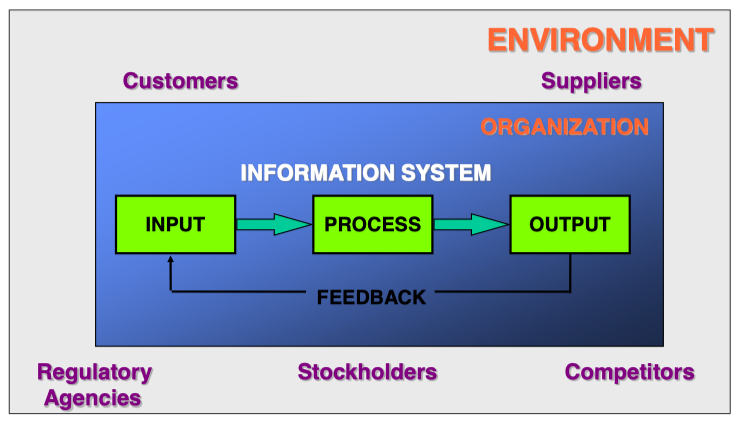
\includegraphics[width=\linewidth]{images/IS_HLM.png}
  \caption{IS High Level Model}
  \label{fig:IS_HLM}
\end{figure}
The blocks are:
\begin{itemize}
  \item Input: Capture or collection of raw data from within the organization of from its external enviroment for processing in an information system.
  \item Output: Distribution of processed information to the people who will use it or to the activities for which it will be used.
  \item Processing: conversion, manipulation and analysis of raw innput into a form that is more meaningful to humans.
  \item Feedback: Output that is returned to the appropriate members of the organization to help them evaluate or correct input.
\end{itemize}

\subsection{Process Analysis: Example}
The production department of a medium-sized company needs to place orders for raw materials, required to feed the production processes.\\
Such raw materials have to be:
\begin{itemize}
  \item Ordered (Negotiation p, Q, T; provided selection, coordination with production needs)
  \item Examined to verify quality
  \item Stored in the warehouse
  \item Registered in the accounting system
  \item Payed
\end{itemize}
With these situation 8 actors are involved in the scenario:
\begin{enumerate}
  \item \textbf{Production}: Requires raw materials needed for productions plans from the warehouse.
  \item \textbf{Warehouse}: When the raw material is not available, first make a request to the purchase office; once the order has been received checks the quality, conformance to request, and stores it.
  \item \textbf{Purchase} office: in charge of negotiating price, quantity, and delivery time with different suppliers.
  \item \textbf{Supplier}: the one chosen to fulfill the order, must deliver the raw materials to the warehouse, and possibly get back the portion not complying with the specifications.
  \item \textbf{Quality} assurance: monitors the efficiency and quality of suppliers by producing statistics for the management.
  \item \textbf{Accounting}: check the orders, receive the delivery receipt from the warehouse, ask the finance department to execute the payment of the supplier invoice, records all transactions.
  \item \textbf{Finance} department: fiscally performs the payment to the supplier and then informs the accounting.
  \item \textbf{Manager}: is a role external to the individual business process that supervises the good working of the enterprise system and controls the economical efficiency. Needs information to take decisions.
\end{enumerate}
The following graph is the rappresentation of the flow:
\begin{figure}[H]
  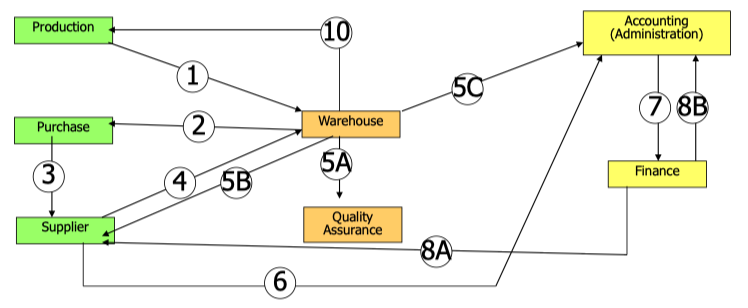
\includegraphics[width=\linewidth]{images/flow.png}
  \label{fig:flow}
\end{figure}
Each step is an activities:
\begin{enumerate}
  \item Production asks warehouse for raw materials
  \item Warehouse has not RM and forwards a request to the purchase office
  \item Purchase office negotiates with the chosen supplier, price quantity and delivery. Issue the order ad send a copy to the accounting department
  \item Supplier delivers the materials to the warehouse together with delivery note
  \item \begin{enumerate}
    \item Warehouse checks received materials and send report to Quality Assurance
    \item Warehouse returns possibly defective goods to supplier
    \item Accounting receives a copies of delivery notes and amount of return materials
  \end{enumerate}
  \item Supplier sends invoice to accounting
  \item Accounting checks invoice and ask finance to procede with payment
  \item \begin{enumerate}
    \item Finance execute payment to suppliers
    \item Finance inform accounting of payments
  \end{enumerate}
  \item Warehouse sends the materiaals to production that ca start operations
\end{enumerate}
The goal of IS is to transmit information (real time), document (past and present) and monitoring (past and present). The more people and locations are involved, the more an IS is required.\\
Another good example is the one of Mc Donald's and Burger King on the slides.\\

Information and Data are different, information is shaped into a form that is meaningful and useful to human beigns in processes such as a decision making. Data is astream of raw facts representing events occurig in organizations or the physical environment before they have been organized and arranged into a form that people can understand and use.
Infomations are also:
\begin{itemize}
  \item Intangible
  \item Not destroyed by usege
  \item Null marginal production costs
  \item Its usage is associated both to the whole organization and to the tasks performed by individuals
\end{itemize}
In organizations:
\begin{itemize}
  \item In organizations there are both information scarcity and information overload
  \item The problems concern all the life cycle: acquisition, storage, retrieval,
  \item There are information obsolescence / perishability risks that affect its change of value in time
\end{itemize}

There are some issue with technnology changes, like fashionable trends:
\begin{itemize}
  \item "Last version syndrome"
  \item "Modernn Times Syndrome"
  \item "Internet Syndrome"
  \item "CRM Syndrome"
\end{itemize}
There are some economy issue: "It doesn't interest me much", Efficacy: "The user must learn hot to use it and not resist the change"

\subsection{IT Models}
The IS are built following 3 main models:
\begin{itemize}
  \item Application: Describes the software architecture. Three layers:
  \begin{itemize}
    \item Presentation: Interaction with end user via GUI
    \item Business Rules: Algorithm and rules to process, control and extract data
  \end{itemize}
  \item Technological: Describes the hardware architecture
  \item Functional: What IS should do, abstracting from how it can be done
  \begin{itemize}
    \item Processes: CRASO, BPMN, UML Activity Diagram
    \item Data: UML Class Diagram, Entity Relationship Diagram
    \item Interaction: Use cases
  \end{itemize}
\end{itemize}
%--------------------------------
%         END SLIDE 01          |
%--------------------------------












\end{document}
